% #############################################################################
% ######################################################## Van Allen Probe Data
% #############################################################################

\chapter{Data}
  \label{ch_data}

Some data is shown in \cref{fig_mode_all_sharp} --- look how great it is! 

Also, check out \cref{tab_iaga}, an example table. These values come from
Jacobs\cite{jacobs_1964}. 

\begin{longtable}{cccccccc}
  \caption[IAGA Magnetic Pulsation Frequency Bands]
    {IAGA Magnetic Pulsation Frequency Bands}
  \label{tab_iaga} \\
  \toprule
  & Pc1 & Pc2 & Pc3 & Pc4 & Pc5 & Pi1 & Pi2 \\
  \midrule
  \endfirsthead
  \bottomrule
  \endlastfoot
  Period (\si{\second}) & 0.2--5    & 5--10    & 10--45  & 45--150 & 150--600 &
    1--40    & 40--150 \\
  Frequency (\si{\mHz}) & 200--5000 & 100--200 & 22--100 & 7--22   & 2--7     &
    25--1000 & 7--25 \\
\end{longtable}

\begin{figure}[!htb]
  \centering
  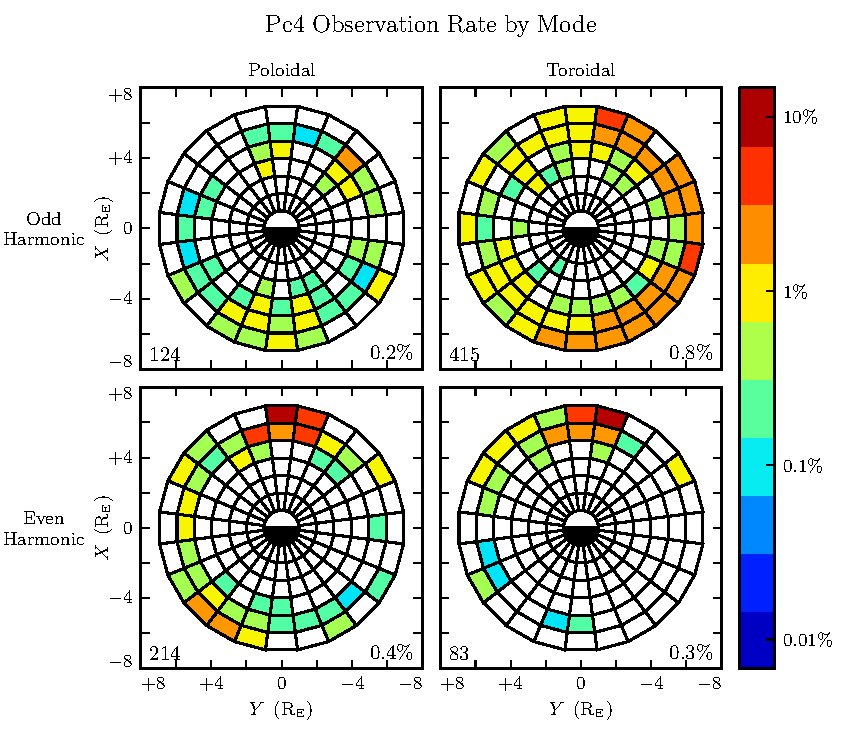
\includegraphics[width=\textwidth]{figures/mode_all_sharp.pdf}
  \caption[Observation Rate of Pc4 Events by Mode]{
    The above figure shows the spatial distribution of Pc4 events observed by
    the Van Allen probes, partitioned by harmonic and polarization. Event
    counts are given in the bottom-left corner. Rates are normalized according
    to the amount of sampling in each bin. Mean rate (assuming a uniform
    spatial sampling) is shown in the bottom-right corner. 
  }
  \label{fig_mode_all_sharp}
\end{figure}
